% !TEX encoding = UTF-8 Unicode
\documentclass[fleqn,twoside]{article}
\usepackage[ngerman]{babel}
\usepackage[utf8]{inputenc}
\usepackage[T1]{fontenc}
\usepackage{graphicx}
\usepackage{fancyhdr}
\usepackage{amssymb}
\usepackage{amsmath}
\usepackage{cite}
\usepackage{eurosym}
\usepackage{wrapfig}
\usepackage{tabularx}
\usepackage{pdfpages}
\usepackage{nicefrac}
\usepackage{wasysym}
\usepackage{multirow}
\usepackage{pifont}
\usepackage{textcomp}
\usepackage{comment}
\usepackage{units}
%\usepackage{siunitx}
\usepackage{yfonts}
\usepackage{calligra}
\usepackage{csquotes}
%\usepackage{emerald}
\usepackage{titlesec}
\usepackage{tikz}
\usepackage{stanli}
\usepackage{romanbar}
\usepackage{graphicx}
\usepackage{tabto}
\usepackage{todonotes}
%\usepackage{3dstructuralanalysis}
%\usepackage{structuralanalysis}
\usepackage{enumitem}
\usepackage{booktabs}
\usepackage{float}


%Befehle abändern
%Itemize ohne Lücken
\setlist[itemize]{noitemsep, topsep=2pt}
\raggedbottom
%\renewcommand{\todo}[1]{\todo[inline]{#1}}


%Betragsfunktion
\newcommand{\abs}[1]{\ensuremath{\left\vert#1\right\vert}}
%Einheitenfunktion
\newcommand{\un}[2]{{\unit[#1]{\color{black!100}[#2]}}}

\usepackage[pdftex, colorlinks, linkcolor=black, frenchlinks]{hyperref}
\usepackage[a4paper , lmargin = {2.5cm} , rmargin = {2cm} , tmargin = {2.5cm} , bmargin = {2.5cm} ]{geometry}
\pagestyle{fancy}
\setlength{\headheight}{12.51453pt}

\title{\Huge{\textfrak{Theoretische Bodenmechanik\\ mit} \textit{Mathematica}\textfrak{ \\Formelsammlung}}}
\author{\calligra{Jonathan C. Walter, Jonas H. Konrad}}
\date{\textfrak{\today}}

%Wir wissen, dass das unit-package veraltet ist. Kann jemand bei Gelegenheit fixen ;)

\begin{document}
\parindent 0pt
\fancyhead[L]{Jonathan C. Walter, Jonas H. Konrad}
\fancyfoot[L]{\frakfamily J. C. W.;J. H. K.}
\fancyfoot[R]{\frakfamily }
\fancyfoot[C]{\frakfamily Wir machen mit Mathematica \\Seite \thepage}
\maketitle \thispagestyle{empty}
%\initfamily %Für Initialien
\begin{center}
\textfrak{Diese Formelsammlung wurde im Sommersemester 2022 von Jonathan Walter und Jonas Konrad verfasst.\\Kein Anspruch auf Vollständigkeit oder Fehlerfreiheit.\\LaTex Vorlage: github.com/Neowise33}
\end{center}
\tableofcontents
%\listoftodos
\newpage

\section{Theoriefragen}

\begin{itemize}
\item Welchen ungünstigen Effekt kann für die Standsicherheit ein Rüttler (=Vibration) an der
Baugrubensohle verursachen?\\
$\blacktriangleright$ Unter (fast) undränierten Bedingungen findet eine Relaxation des effektiven Spannung statt. Der
Erdwiderlager wird zusätzlich (neben der Strömungskräften) abgeschwächt.
\item Nach Ausfall einer Aussteifung wurde die Baugrube von oben geflutet. Nach der Reparatur wurde die Baugrube wieder gelenzt. Welche Gefahr kann dabei für ein provisorisches Fundament auf der Baugrubensohle entstehen wenn der Wasserspiegel in der Baugrube zu schnell abgesenkt wird und wenn die Sättigung des Schluffs bis 1m unter der Sohle nicht garantiert ist?\\ 
$\blacktriangleright$ Luftblasen vergrößern das Volumen und verdrängen langsam Wasser. Dadurch kann sich der PWD unter der Sohle nicht sofort abbauen und große Gradienten können zur Bodenverflüssigung führen .
\item Porenwasserüberdruck nach Absenkung des Wasserspiegels:\\
$\blacktriangleright$ Fall a) Infolge einer schnellen Absenkung des Wasserspiegels ändert sich die effektive Spannung
im Boden nicht, also entstehen keine Verformungen, also ist kein Wassertransport nötig. Kein Porenwasserüberdruck
wird sich bilden. Der PWD ändert sich sofort.\\
$\blacktriangleright$ Fall b) Infolge einer schnellen Absenkung des Wasserspiegels ändert das Volumen der Luftblasen
und findet ein Wassertransport statt. Wasser wird nach oben Verdrängt und eine Strömungskraft
entsteht dabei. Ein Überdruck von 10 kPa kann nur bei extrem kleiner Durchlässigkeit bzw. bei
großem Anteil an der Luftblasen entstehen.
\item Welchen ungünstigen Effekt kann der Herstellungsprozess (z.B. durch Rammen oder mit
Vibration) von Palisaden (Pfosten Stabilisierung Rutschhang) haben?\\
$\blacktriangleright$ Infolge der Vibration findet eine Verdichtung statt. Damit:
\begin{itemize}
 \item steigt der Grundwasserspiegel
 \item wird die Kapillarspannung kleiner
 \item bleibt die Strömungskraft unverändert
\end{itemize}
\item Schlagen Sie ein Warnsystem und eine Vorbeugung der Rutschung eines Schräghangs vor.\\
$\blacktriangleright$ Man soll die Lage des Grundwasserspiegels besonders nach Niederschlägen beobachten
und für evtl. Entwässerung des Hangs sorgen (Dränage, Pflanzen).
\item Wie ändert sich der Grundwasserspiegel, die Kapillarspannung und die Strömungskraft infolge
einer Verdichtung (z.B. nach einer Vibration aus einer Verkehrslast)?\\
$\blacktriangleright$ Nach einer Vibration kann der GWSp nicht weiter steigen, aber Grundwasser kann
aussickern. Die Kapillarspannung wird nicht entstehen. Die Richtung der Strömungskraft wird flacher
geneigt.
\item Welche praktische Folgen hätte die Verletzung des Festigkeitskriteriums am Punkt A für das
Fundament? Was würden Sie als Indikator einer Rutschungsgefahr für diesen Hang empfehlen?\\
$\blacktriangleright$ Man soll den ganzen Bruchmechanismus analysieren. Eine punktuelle Verletzung
des Bruchkriteriums kann durch die Umverteilung der Scherbeanspruchung aufgehoben werden.
Man soll die Verschiebungen des Fundaments beobachten.
\item Wie kann die Beziehung zwischen dem Wassergehalt und der undräniertenten
Festigkeit eines stark überkonsolidierten Tons durch die Mikrorisse beeinflusst werden?\\
$\blacktriangleright$ Die Mikrorisse können einen viel größerenWassergehalt (und damit auch eine viel größere Porenzahl)
haben und so für die Festigkeit der stark überkonsolidierten Tonprobe entscheidend sein.
\item Obere Abschätzung Halt eines Hangs?\\
$\blacktriangleright$ Falls assoziierte Fließregel (AFR: $\psi = \varphi$) und kinematische Lösung verwendet wird. (Untere Abschätzung NAFR: $\psi\neq\varphi$ und Statische Lösung)
\item Wie muss die Vakuum-Vorbelastung für eine dickere Kriechscholle angepasst werden?\\
$\blacktriangleright$ Vakuum-Vorbelastung erhöhen und somit auch den OCR-Wert.
\item Wie könnte die Gefahr einer Verflüssigung durch eine PWD-Messung in situ kontrolliert wer- den? Wie groß (und wann gemessen: zwischen Achsen oder unter der Achse) wäre der PWD, der der vollständigen Bodenverflüssigung $\sigma_v = 0$ entspricht?\\
$\blacktriangleright$ Der PWD soll nach der Durchfahrt eines Fahzeugs gemessen werden. Die Verflüssigung also die eff. Spannung $\sigma = 0$ erfordert $u = \sigma_{\text{ges}}$, wobei $\sigma_{\text{ges}}$ die Gesamtspannung aus dem Eigengewicht bezeichnet.
\end{itemize}

\section{Allgemeine Annahmen/Gesetzmäßigkeiten}

%\subsection{Einheitenumrechnung}

%\begin{itemize}
%\item $Nm = \unit{\frac{kg \cdot m}{s^{2}}}$
%\end{itemize}

\begin{itemize}
\item Ablauf Spannungsverlauf:
	\begin{enumerate}
		\item Boden mit vorhandenen Spannungen
		\item Nach Probeentnahme: $\sigma^{ges}=u+\sigma = 0$ ; $\sigma$ unverändert
		\item Nach Einbau in Triax und schneller Belastung (undräniert): $\sigma$ unverändert ; $\sigma^{ges}$ = vorhandene Spannung + vorgegebener Wert ; $u=\sigma^{ges}-\sigma$
		\end{enumerate}
\item Bei langsamer Scherung im Wasserbad (dräniert) baut sich kein Porenwasserdruck auf: $u$ = 0
\item $K_0 = 1$ statt $K_0=1-\sin(\varphi)$ als legitime Annahme bei überkonsolidierten Boden 
\end{itemize}

\section{Allgemeine Formeln und Zusammenhänge}

\subsection{Bodenparameter und Spannungen}

\begin{itemize}
	\item $e=\frac{w \gamma_s}{\gamma_w}$
	\item $\gamma' = \frac{(\gamma_s-\gamma_w)}{(1+e)}$ oder $\gamma' = \gamma - u$
	\item Wichte $\gamma'$ unter Auftrieb:
	\begin{itemize}
		\item  S=1: $\gamma' = (\gamma_s - \gamma_w)(1-n)$
		\item  S<1: $\gamma' = (\gamma_s - \gamma_w)(1-n_w) - \gamma_s n_a$ ; $n_a = (1-S)n$
	\end{itemize}	 
		
	\item $\gamma = \gamma'+\gamma_w$
	\item $OCR$ = $\frac{\sigma_V}{ \sigma_{eff}} > 1 =$ überkonsolidiert 
	\begin{itemize}
		\item $\sigma_V$ = Vorbelastungsspannung 
		\item $\sigma_{eff}=\sigma_v \cdot \tan(\varphi_s)$
	\end{itemize}
	\item Gleitkeil Abschätzung: $\vartheta = 45 - \frac{\varphi}{2}$
	\item Effektive (Anfangs-)Vertikalspannung:
	\begin{itemize}
		\item In trockenem Boden $\sigma_{v0}=h_{\gamma}\cdot \gamma$
		\item In kapillar durchfeuchtetem Boden mit oben aufliegender trockener Bodenschicht:\\ $\sigma_{v0} = h_{\gamma} \cdot \gamma + (z-h_{\gamma})\gamma'+ h_c \gamma_w $
		\item Unter GWSp mit oben aufliegender trockener Bodenschicht: $\sigma_{v0} = \gamma'(Z+h_c)+\gamma_w\cdot h_c+h_{\gamma}\cdot\gamma	$
		\begin{itemize}
			\item $z$ Gesuchte Tiefe ab GOK
			\item $Z$ Gesuchte Tiefe ab GWSp
		\end{itemize}
	\end{itemize}
	\item Effektive (Anfangs-)Horizontalspannung: $\sigma_{h0} = K_0 \sigma_v$
	\item Effektive Wiederbelastungs horizontal Spannung: $\sigma_h=\sigma_{VB}\cdot K_0-K_U\cdot (\sigma_{VB}-\sigma_v)=\sigma_{VB}\cdot K_0-\frac{\nu}{1-\nu}(\sigma_{VB}-\sigma_v)$
	\item Anfangsporenwasserdruck: $u_0 = (z-z_{GWSp}) \cdot \gamma_w$
	\item Gesamtspannung: Vertikal und Horizontal zu Spannung aus Erddruck Porenwasserdruck addieren
	\item Scheinbare Kohäsion aus Kapillaritätsdruck: $c = \frac{1}{2} M_c p_c$
	\item Bodenparameter mitteln:
	\begin{itemize}
		\item Kohäsion: $\overline{c} = \frac{h_1 c_U + h_2 c_T}{\sum h_i}$
		\item Reibung: $\overline{\tan \varphi} = \frac{G_1 \tan(\varphi_U) + G_2 \tan(\varphi_T)}{G_1 + G_2}$
		\item Wichte: $\overline{\gamma} = \frac{G_1 + G_2}{\sum A_i}$
	\end{itemize}
\end{itemize}

\subsection{Ödometer}

\begin{itemize}

	\item Kompressionsdiagramm auswerten (Abszisse: $\sigma$ ; Ordinate: 1+$e$)
	\item $e=\frac{w \cdot \gamma_s}{\gamma_w}$ ; w = Wassergehalt in \%
	\item äquivalente Hvorslev-Spannung $\sigma_e$: mit e waagrecht mit Erstbelastungslinie, $\sigma$ ablesen.
	\item $\kappa_B = - \frac{ \log\left(\frac{(1+e)_1}{(1+e)_2}\right) }{  \log\left(\frac{\sigma_1}{\sigma_2}\right) }$ $\rightarrow$ Wiederbelastung $\rightarrow$ Auf oberen flachen Teil durchführen
	\item $\lambda_B = -\frac{ \log\left(\frac{(1+e)_1}{(1+e)_2}\right) }{ \log\left(\frac{\sigma_1}{\sigma_2}\right) }$ $\rightarrow$ Auf steilen Teil durchführen $\rightarrow$ Erstbelastung
    \item Dehnung: $\Delta\epsilon=\frac{\Delta e}{1+e}$
	\item Für Punkt $z$ den Wert $e$ berechnen; $\sigma$ aus Diagramm ablesen; $c_u = \sigma_{VB} \tan(\varphi_s)$
	\item Analytische Lösung:
	\begin{itemize}
	    \item $\ln\left[\frac{e}{e_{e0}}\right]$ = $\lambda_B \ln\left[\frac{\sigma_{VB}}{\sigma_{e0}}\right]$
	    \item $\ln\left[\frac{e}{e(z)}\right]$ = $\kappa_B \ln\left[\frac{\sigma_{VB}}{\sigma(z)}\right]$
	\end{itemize}
	\item $OCR = \frac{\sigma_e}{\sigma_{eff}} (\sigma_{eff} = \sigma')$
	\item undränierte Kohäsion: $c_u = \sigma_e \tan(\varphi_s)$
	\item effektive Kohäsion: $c' = \sigma_e(\tan(\varphi_s - \tan(\varphi')))$
	\item $\rightarrow e_{e0} \& \sigma_{e0}$ von $\lambda$ (steilen) Gerade ablesen. Einen Punkt wählen.\\
		$\boxed{\Rightarrow \sigma_{VB}(e,\sigma) = \sigma_{e0} \left( \frac{\sigma_{e0}}{\sigma}\right)^{\frac{\kappa}{\lambda-\kappa}} \exp\left( \frac{e_{e0}-e}{\lambda-\kappa} \right)}$\\
	\item Porenwasserdruckänderung: $\Delta u=B\frac13\Delta q+A\Delta q$
	\begin{minipage}{0.5\textwidth}
	        \item Graphische Möglichkeit zur Bestimmung $\sigma_{VB}$:
	\end{minipage}
	\begin{minipage}{0.5\textwidth}
	    \includegraphics[width=0.6\textwidth]{Grafiken/Ödometer_graphisch}
	\end{minipage}
	\item Praktische Anwendung bei Setzungsberechnung durch Auflast:
	\begin{enumerate}
	    \item Grundsätzlich Punkt (x/y)=($\sigma_{eff}/e$), davon ausgehend die flache Wiederbelastungslinie bis Erstbelastungslinie zeichnen
	    \item 3 Fälle:
	    \begin{itemize}
	        \item Nur Wiederbelastung: $\Delta e = \kappa \ln(\frac{\sigma_{eff}+\sigma_{Auflast}}{\sigma_{eff}})$ 
	        \item Nur Erstbelastung: $\Delta e = \lambda \ln(\frac{\sigma_{eff}+\sigma_{Auflast}}{\sigma_{eff}})$
	        \item Gemischt: Aus Diagramm ablesen $\rightarrow$ Pfad folgen von $\sigma_{eff}$ aus und $\Delta e$ ablesen.
	    \end{itemize}
	    \item $s = \int_0^z \Delta \epsilon dz = \sum e_{Schicht} \cdot h_{Schicht} $
	\end{enumerate}
	
	
	
\end{itemize}

\subsection{Konsolidierung}

\begin{itemize}
	\item Barotrope Steifigkeit: $E_s=\frac{\sigma_{v0}}{\kappa}$
	\item Konsolidierungsbeiwert: $c_v=\frac{kE_s}{\gamma_w}$
	\item Dimensionsloser Zeitfaktor: $T_v=\frac{c_vt}{H^2}$ ; $\un{t}{s}$; $\un{h}{m}$; $H$ = Drainageweg Wasser ;
	\item Verfestigungsgrad: $\bar{\mu}\approx 2 \cdot \sqrt{T_v/\pi}$
	\item Konsolidierungsgrad: $\mu=\frac{1}{2}(3\bar{\mu}-1)$ ; Faktor Verfestigung Boden nach t Sekunden aus $T_v$
	\item Aufgebauter Porenwasserdruck nach $n$ Zyklen$\cdot$Konsolidierungsgrad \\= Porenwasserdruck nach t$\cdot$n Wartezeit; 
		$(\Delta u \cdot n) \cdot \mu = \Delta u_{konsolidiert}$
\end{itemize}

\subsection{Krey-Tiedemann}\label{Scherversuch}
		
\begin{minipage}{0.35\textwidth}
\begin{itemize}
	\item Allgemeine Formeln:
	\begin{itemize}
		\item $c_u \approx \sigma'_{VB} \tan(\varphi_s)$
		\item $w(z)= \frac{\rho_w V_p}{\rho_s V_s}=e \frac{\rho_w}{\rho_s}$
		\item$\sigma_{11}=x \cdot \gamma' \cdot \beta$
		\item$\tau = \sigma_{11}  \cdot \frac{\sigma}{\sigma'} \cdot \tan(\beta)$
	\end{itemize}
	\item Ablauf Krey-Tiedemann:
	\begin{enumerate}
		\item $\varphi_s$ auftragen
		\item $\sigma_{VB}$ auftragen und bis $\varphi_s$ verlängern
		\item An Schnittpunkt $\varphi '$ ansetzen und nach links einzeichnen
		\item mit $\varphi$ und $\alpha$ den Schnittpunkt mit $\varphi_s$ bestimmen.
		\item Dieser Punkt ist $\tau_{\max}$ und mit dem gegebenen $\sigma$ wird ein Kreis innerhalb der $\varphi '$ konstruiert.
		\item Schnittpunkt rechte Seite Kreis mit Abszisse ist $\sigma_1$
	\end{enumerate}
\end{itemize}
\end{minipage}		
\begin{minipage}{0.6\textwidth}
	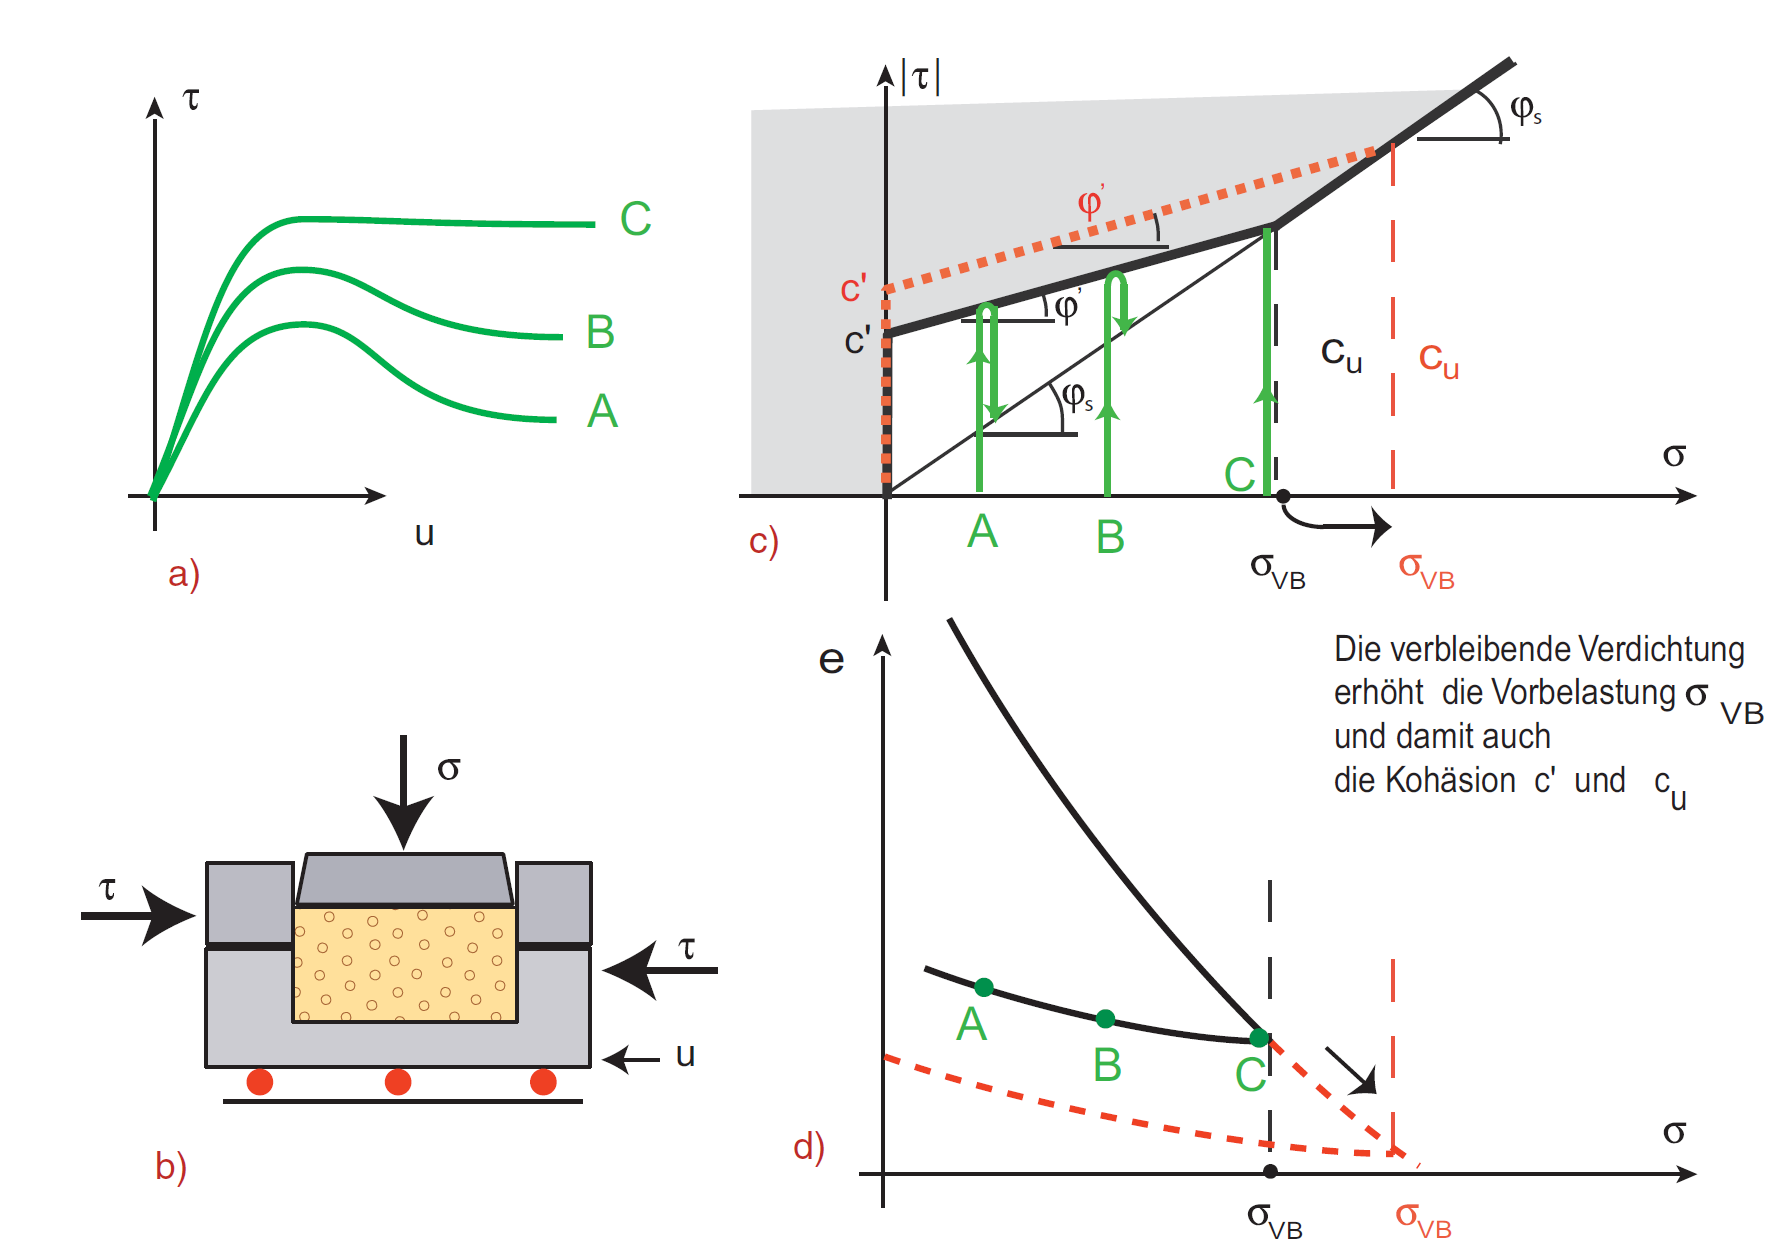
\includegraphics[width=1\textwidth]{Grafiken/Krey-Tidemann-Kriterium.png}
\end{minipage}


\subsection{Mohr'scher Spannungskreis}
\begin{itemize}
    \item Reibungswinkel in schwachen Querschnitt:
    \begin{itemize}
        \item $\tan(\varphi) = \frac{h}{s+r\cos(\varphi_{(steilster)})}$ ; $h=r\sin(\varphi_{(steilster)})$ ; $s=\frac{1}{2}(\sigma_{1,max}+\sigma_3)$ ; $r=\frac{1}{2}(\sigma_{1,max}-\sigma_3) $
    \end{itemize}

	\item$\sigma_{11} \& \sigma_{21}$ bekannt, $\sigma_{11,(min)} \& \sigma_{22,(max)}$ gesucht:
	\begin{itemize}
	\item Möglichkeit 1 - rechnerisch:
	\begin{itemize}
	    \item $r^2 \leq m^2 \sin(\varphi)^2$ ; $r^2 = (\sigma_{11} - \sigma_{22})^2 + \sigma_{12}^2$ ; $m = \frac{1}{2} (\sigma_{11}+\sigma_{22})$
	\end{itemize}
	\item Möglichkeit 2 - graphisch:
		
		\begin{enumerate}
		\item Mit c und $\varphi_{\text{(des Bodenmaterials)}}=\arctan\left(\frac{\tau}{\sigma}\right)$ Schergerade einzeichnen.
		\item Bekannten Punkt mit $\sigma_{11} \& \sigma_{21}$ einzeichnen.
		\item Durch den Punkt mit Winkel des Hangs Gerade ziehen.
		\item Kleinsten und größten Kreis einzeichnen. Schnittpunkt mit Gerade aus 3. einzeichnen
		\item Senkrechte auf 3. von den Schnittpunkten aus nach unten rechts bis sich mit Kreis schneidet.
		\item Neuen Schnittpunkte geben: $\sigma_{11,(min)} \& \sigma_{22,(max)}$ an.
		\end{enumerate}
	\item Zusätzliche Belastung graphische Ermittlung $\phi_{erf,neu}$:
\end{itemize}
\end{itemize}
    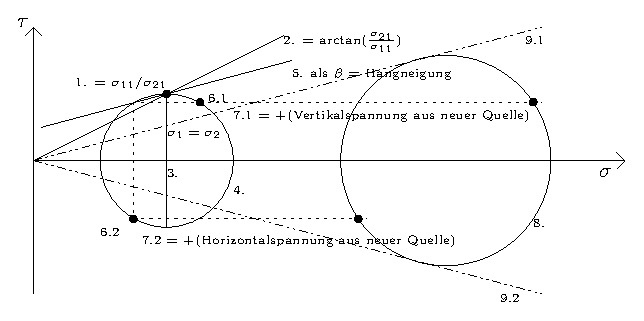
\includegraphics[width=1\textwidth]{Grafiken/Spannung_aus_Fundament_(Mohrscher).eps}


\subsection{Skempton Parameter}

\begin{itemize}
	\item $B = \frac{\Delta u}{\Delta p^{ges}}$ ; aus B-Test, tendenziell steigen $\sigma_1 und \sigma_3$
	\item[$\rightarrow$] B beschreibt Qualität der Sättigung. Perfekt gesättigte Triaxialproben: $B = 1$
	\item $A  = \frac{\Delta u - B \Delta p^{ges}}{\Delta q}$ ; $\sigma_1$ oder $\sigma_3$ steigen an. Wenn $B=1: A=-\frac{\Delta p}{\Delta q}$
	\item $\tab$ $\Delta q = q_{1,2 Ende}-q_{1,2 Anfang}$ ; $q=\abs{\sigma_1 - \sigma_3}$
	\item $\tab$ $\Delta p=\Delta tr\sigma^{ges} = \frac{\sigma_1 +2\cdot \sigma_3}{3}_{\text{(Zustand 2)}} - \frac{\sigma_1 +2\cdot \sigma_3}{3}_{\text{(Zustand 1)}} $
	\item Für $p^{ges}$ = const. $\rightarrow$ pro Zyklus $\Delta u=2Aq^{ampl} = 2A(\Delta \sigma^{ges}_v - \Delta \sigma^{ges}_h)$ ; $\Rightarrow$ kumulativer Anstieg
	\item Für $q$ = const. $\rightarrow$ pro Zyklus $\Delta u=B\Delta p^{ges}$ ; Kurze Belastungsdauer, Gesamtspannung bleibt gleich: $\Delta \sigma_v = -\Delta u$
\end{itemize}

\subsection{Triaxialversuche}

\begin{itemize}
	\item triaxiale Kompression ($\sigma_1 > \sigma_3$) $\rightarrow$ $M_C$ ist maßgebend
	\begin{itemize}
	    \item $M_C=\frac{6\sin(\varphi')}{3-\sin(\varphi')} = \frac{q}{p}$
	\end{itemize}
	\item triaxiale Extension ($\sigma_3 > \sigma_1$) $\rightarrow$ $M_E$ ist maßgebend
	\begin{itemize}
	    \item $M_E=-\frac{6\sin(\varphi')}{3+\sin(\varphi')}$
	\end{itemize}
	\item $\dot{p}^{ges}=\frac{1}{3}(\dot{\sigma}_1^{ges}+2\dot{\sigma}_3^{ges})$
	\item $\abs{\dot{q}}=\abs{\dot{\sigma}_1-\dot{\sigma}_3}$
	\item $\dot{u}\approx B\dot{p}^{ges}+A \abs{\dot{q}}$
	\item $\Delta p$ und $\Delta q$ berechnen: $A$ und $B$ bekannt, $p,q,u$ ebenso:
	$\Delta p = (1-B) \frac{1}{3} \Delta q-A\Delta q$ ;
	$q+ \Delta q = M_c(p+\Delta p)$
	$\boxed{\Leftrightarrow \Delta q=\frac{q-M_cp}{M_c\left(\frac13(1-B)-1\right)-1}}$
	\item Kohäsion aus A und B berechnen
	
\begin{minipage}{0.5\textwidth}
	\item Bekannte Steigung aus $\varphi_s \rightarrow M_C \text{ oder } M_E$
	%	$M_{c,neu}$ vorgehen:\\ 
	\begin{enumerate}
		\item $M_{c,\text{vorläufig}} = \Delta_{s}(aus \varphi_s) \cdot B$ 
		\item $M_{c,neu} = \frac{\Delta_{s,\text{Zähler} \overset{!}{=} 1} - \Delta_{s,\text{Nenner}} \cdot A}{\Delta_{s,\text{Nenner}}}$
		\item Ab $p = \sigma_{a0}$ auftragen
		\item Schnittpunkt aus $M_c = M_{c,neu}$ berechnen.
		\item $c_u = \frac{q}{2}$
	\end{enumerate}
\end{minipage}		
\begin{minipage}{0.4\textwidth}
	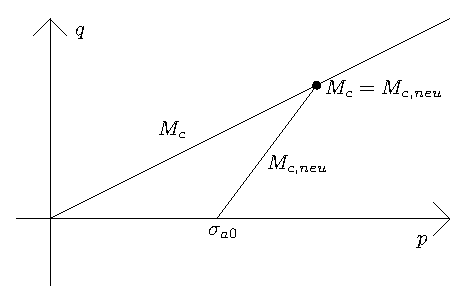
\includegraphics[width=1\textwidth]{Grafiken/Graphische_Version.eps}
\end{minipage}
    \item $M_c = \dfrac{q_A + \Delta q}{p_A + \frac{1}{3} \Delta q - \Delta u}$
	\item Abschätzung maximale Schubspannung: $\tau_{\max} = \sigma_V \tan(\varphi')+c'$\\
	$\sigma_V$ aus Angabe Belastung Knick nehmen.
	\item Restscherfestigkeit: $\tau = \sigma \tan(\varphi_s)$ ; $\sigma$ aus in-situ
	\item Winkel Gesamtscherfestigkeit (Kompression): $\sin(\varphi_s)=\frac{\sigma_1-\sigma_3}{\sigma_1+\sigma_3}$ \\
	mit effektiver Spannung ($p$,$q$) berechnen!
	\item Winkel Gesamtscherfestigkeit (Extension): $\sin(\varphi_s)=\frac{\sigma_3-\sigma_1}{\sigma_3+\sigma_1}$
	\item $\sigma_{1,\text{peak}}-\sigma_{3}'=(\sigma_{1,\text{peak}}+\sigma_{3}')\sin(\varphi')+2c'\cos(\varphi')$
	\item Undrainierte Schubsteifigkeit: $G= \frac{\Delta q}{3 \Delta \epsilon_q}$
	\item Volumendehnung: $\epsilon_{v}=\epsilon_1 + 2\epsilon_3$
	\item Deviatorische Dehnung: $\epsilon_q = \frac{2}{3}(\epsilon_1 - \epsilon_3)$
	$\rightarrow$ Bei undränierten Versuchen gilt: $\epsilon_{2(3)}=-\frac{\epsilon_1}{2}$
	\item UU-Rahmenscherversuch
	\begin{itemize}
	    \item Stich-Kriterium: $\sigma_1 = \sigma_2 + \frac{2}{\sin(2 \alpha)} c(\alpha)$ ; $\alpha =$ Winkel Scherfuge
	    \item Richtungsabhängige Kohäsion: Bsp: $c_u(\alpha) = 100 \cos(\frac{2}{3} \alpha)$
	\end{itemize}
\end{itemize}

\subsection{Kriechhang, Verdübelung, Verankerung}
		
\begin{itemize}
	\item Schubfestigkeit oberhalb Kontaktfläche (ohne Verdübelung): $\tau_\alpha = F_1 + G_1 \sin(\beta)$
	\item $h$ senkrecht zur Böschung: $\tau_\alpha = \gamma_w h \cos(\beta) \sin(\beta) + h \gamma' \cos(\beta) \sin(\beta)$
	\begin{itemize}
		\item $G =$ Gewicht einer vertikalen Bodensäule mit Einheitsfläche 1 m$^2$ gemessen entlang der Böschung (und nicht horizontal); 		
		\item $F =$ Sickerkraft in dieser Bodensäule
	\end{itemize}
	\item Allgemeiner Ansatz nach Leinenkugel:
	\begin{itemize}
	    \item $c_u = c_{u\alpha}\left(1+I_V\ln\frac{\dot{\gamma}}{\dot{\gamma}_\alpha}\right)$ ; $\dot{\gamma} = \frac{[[\dot{u}]]}{d}$ ; $\dot{\gamma}_\alpha = \frac{[[\dot{u}]]_\alpha}{d}$ ; wobei gilt: $c_{u\alpha}=\tau_\alpha$
	    \item $c_{u,erf} = c_{u\alpha}(1+I_V\ln\left(\frac{[[\dot{u}]]}{[[\dot{u}]]_\alpha}\right)$
	\end{itemize}
	\item Erforderliche Schubkraft nach Leinenkugel (an Sohle): $\tau = \tau_\alpha \left( 1+ I_v \ln \left( \frac{1}{n-\text{fach langsamer}} \right) \right) = \tau_{\alpha} \left( 1+I_v \ln\left(\frac{\dot{\gamma}}{\dot{\gamma_{\alpha}}}\right)\right)$
	\item Schubkraft pro 1m$^2$ Oberfläche der Dübel: $\tau_D = \tau_\alpha - \tau = \tau_\alpha I_v \ln (n-\text{fach langsamer})$
	\item Kraft pro Dübel: $p_f \cdot h= h \left[1+I_v \ln\left(\frac{\frac{v_{red}}{a-D}}{\dot{\gamma_a}}\right)\right] k_0 c_{u\alpha} D = \tau_D a L$ 
	\begin{itemize}
		\item $p_f = \left[1+I_v \ln \frac{v_{red} / (a-D)}{\dot{\gamma_a}}\right] k_0 c_{u\alpha} D$
		\begin{itemize}
			\item $k_0 = 4,83 \cdot \left[ 2,76 \frac{D}{a}+1 \right]$
			\item $c_{u\alpha}=\tau_\alpha$
		\end{itemize}
		\item a = axialer Abstand quer zur Hanglinie
		\item Verformungsrate: $\dot{\gamma}_\alpha = \frac{v}{h_\gamma \cos(\beta)}$
	\end{itemize}
		
	\item Verdübelung eines Hangs, Sicherheitsabstand für Knopflochlösung: $x=v\cdot t$
	\begin{itemize}
		\item $h$=Höhe Gleitscholle, $B$=Breite der Zone, $D$=Durchmesser eines Dübels, $H$=Schubkräfte auf den Seiten, $P_f$ = Wirkung der Verdübelung pro lfm der Böschungslinie (ohne Seitenkräfte)
		\item Kriechrate des Hangs in verdübelter Zone: $v=v_\alpha \exp\left[\frac{c_{u,\text{erf}}-c_{u\alpha}}{I_V c_{u\alpha}}\right] \Leftrightarrow c_{u,\text{erf}} - c_{u\alpha} = I_V c_{u\alpha} \ln\left(\frac{v}{v_\alpha}\right)$
		\begin{itemize}
			\item Referenzkohäsion: $c_{u\alpha}=W\sin(\beta)$
			\item Notwendige Kohäsion: $c_{u,\text{erf}}=\frac{WB\sin(\beta)-P_f+H}{B}$
			\begin{itemize}
				\item $W=\gamma h \cos(\beta)$
				\item $P_f=B(c_{u\alpha}-c_u)=B(I_V \cdot c_{u\alpha} \cdot \ln(0,1))$
				\item $H=2 \cdot 0,1 \cdot c_{u\alpha} h \cos(\beta)$
			\end{itemize}
		\end{itemize}
	\end{itemize}
		
	\item Ausführung mit Vakuum-Vorbelastung 
		\begin{itemize}
			\item n-fache Bremsung der Kriechrate: $n = (\frac{OCR_a}{OCR_b})^{\frac{-1}{I_v}}= (\frac{1}{OCR})^{\frac{-1}{I_v}}$
			\begin{itemize}
				\item $I_v=\frac{\ln\left(\frac{c_{ua}}{c_{ub}}\right)}{\ln\left(\frac{\dot{\gamma_a}}{\dot{\gamma_b}}\right)}$ %$\frac{\dot{\gamma}_a}{\dot{\gamma}_b} = (\frac{c_{ua}}{c_{ub}})^{1/I_V}=(\frac{\tau_{ua}}{\tau_{ub}})^{1/I_V}$ ; $\dot{\gamma}_{a,b}$ = Verformungsraten Boden vorher/nachher\\
				\item $OCR = \frac{\sigma_{11}+\Delta \sigma_{11}}{\sigma_{11}}$
			\end{itemize}
			\item Normale Komponente nach der Belastung: $\sigma_{11,nachher}=\sigma_{11} \cdot OCR$
			\item Schubkomponente: $\sigma_{21} = \sigma_{11} \cdot \sin(\beta)$
			\begin{itemize}
				\item $\sigma_n = \sqrt{\sigma_{11}^2 + \sigma_{21}^2}$
				\item $m=\frac{\sigma_n}{\cos(\beta)}$ ; $r=\sigma_n \cdot \tan(\beta)$ ; $\sigma_1=m+r$ ; $\sigma_2=m-r$ ; $\sigma_3 = \sigma_2$
				\item $p=\frac{(\sigma_1+\sigma_2+\sigma_3)}{3}$ ; $q=\sigma_1-\sigma_2$
    \begin{figure}[H]		
		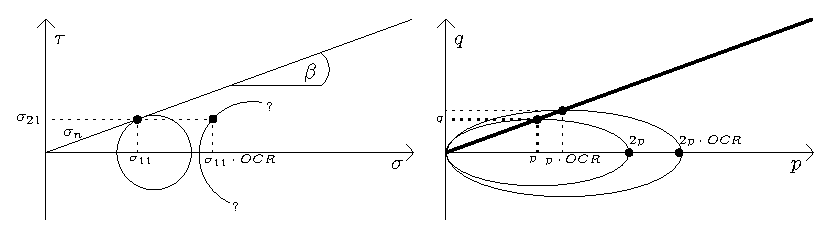
\includegraphics[width=0.8\textwidth]{Grafiken/Konsolidierung_Kriechhang.eps}
		\caption{Links: Mohr'scher Kreis vor und während der Vorbelastung.\\ 
		Rechts: Spannungszustand und Vorbelastungsflächen vor und nach der Vorbelastung}
    \end{figure}
		\end{itemize}
	\end{itemize}
	
\item Reiner Kriechhang / Schräghang
	\begin{itemize}
		\item Spannungsberechnung: ($x_1$ = senkrecht zu Hang gemessen)
		\item $\sigma_{11} = x_1 \gamma' \cos(\beta) + \gamma_w \cdot h_c$
		\item $h_c = z \cdot \cos(\beta)^2$ ; $z$ = Tiefe GWSp unter Oberfläche (vertikal gemessen)
		\item $\sigma_{21} = x_1 \cdot \gamma \cdot \sin(\beta) + j \cdot \gamma_w$
		\item Erforderlicher Reibungswinkel: $\varphi_{\text{erf}} = \arctan(\frac{\sigma_{21}}{\sigma_{11}})$
		\begin{itemize}
		    \item $\stackrel{\text{bei verflüssigten Schräghang}}{========== \Rightarrow} \tan(\varphi_{\text{erf}}) = \frac{\tau}{\sigma^{\text{eff}}} = \frac{\gamma h \sin(\beta)}{\gamma h \cos(\beta)-u}$
		\end{itemize}
		
	\end{itemize}
	
\end{itemize}

\subsection{Wasser im Krafteck und noch mehr}

\begin{itemize}
	\item Strömungskraftdichte und Porenwasserüberdruck
	\begin{itemize}
		\item Hydraulischer Gradient: $i=\frac{\partial h}{\partial l}=\frac{w}{k} \stackrel{\text{(bei langem Hang)}}{=}  \sin(\beta) $
		\item Gradient bei $\Delta h$ des GWSp mit zwei versch. Schichten.
		\begin{itemize}
			\item $w=k_U i_U = k_T i_T$ ; $i_U = \frac{\Delta h}{L_U + \frac{k_U}{k_T}L_T}$ ; $i_T = \frac{k_U}{k_T} i_U$
		\end{itemize}
		\item Allgemeine Formel hydraulischer Gradient mehrere Schichten
		\begin{itemize}
		    \item $\bar{i} = \sum\limits_{i=1}^n = \frac{\Delta h_i}{d_i} = \frac{\Delta H}{\Delta l}$
		    \item $ \bar{k} = \frac{\Delta L}{\sum\limits_{i=1}^n \frac{d_i}{k_i} }$
		    \item $i_i = \frac{\bar{k}}{L_n} \cdot \bar{i} = \frac{\bar{k}}{k_n} \cdot \frac{\Delta H}{\Delta L}$
		    \item Bei sehr großen Unterschieden in der Durchlässigkeit $k_1 \geq 1000 \cdot k_2$ kann angenommen werden, dass nur in der undurchlässigen Schicht Potential abgebaut wird.
		\end{itemize}
		\item Strömungskraftdichte: $j= \gamma_w \cdot i$
		\item Porenwasserüberdruck auf Körper (in Mittelpunkt der Gleitfläche): $u^+=i\gamma_wx_1$
		\item Gewicht mit Strömungskräfte (Auftrieb): $G = A_1 \cdot (\gamma' - j_1) + A_2 \cdot (\gamma' - j_2)$
		\item Verflüssigter Boden: $\sigma^{\text{eff}} = 0 \Rightarrow \sigma^{\text{eff}} = \sigma^{\text{ges}} - u =0 $
	\end{itemize}
	\item Kräftegleichgewicht
	\begin{enumerate}
		\item Mit Strömungskraft
		\begin{itemize}
			\item Eigengewicht: $G=\gamma' \cdot V$
			\item Strömungskraft: $F_s=j \cdot V$
		\end{itemize}
		\item Mit Porenwasserdrücken
		\begin{itemize}
			\item Eigengewicht: $G=\gamma \cdot V$
			\item Hydrostatischer Anteil der Porenwasserdrücke: $U=\gamma_w \cdot V$
			\item Porenwasserüberdrücke: (Summe über Ränder) $U^+=j \cdot V$
		\end{itemize}
		\item Für beide Fälle zu verwenden:
		\begin{itemize}
			\item Reaktionskräfte: Q
			\item Zwischenkräfte: $E_{12}$
			\item Äußere Belastungen
		\end{itemize}
	\end{enumerate}
\end{itemize}

\subsection{Roscoe Invarianten}

\begin{itemize}
	\item $p=\frac{\sigma_1+2\cdot\sigma_3}{3}$ , Auch für $\Delta p^{ges}$ verwenden.
	\item $q=\sigma_1-\sigma_3 \widehat{=} 2 \cdot c_u$
	\item $M_C=\frac{q}{p} = \frac{6s}{3-s}$ ; $s=\sin(\varphi_s)$ ; $\eta$ beschreibt Steigung Schergerade in $p$ - $q$ Diagramm 
	\item $\rightarrow$ (dafür die gesamten Spannungen mit abgezogenen $u_0$ verwenden)
	\item Daraus ergibt sich: $2c_u=\frac{6 \cdot \sin(\varphi)}{3-\sin(\varphi)} \cdot p$
	\item Spannungspfad startet bei: $p_0 = \frac{1}{3} (1+2K_0)\sigma_0$ ; für $\sigma_v^{ges},\sigma_h^{ges}$ durchführen.
	\item Für Startpunkt der zyklischen Belastungen die effektive Spannung ($\sigma_v^{ges},\sigma_h^{ges}$) im Boden benutzen)
		$A$ gibt Steigung von -$p$ Sprung an, $q^{ampl}$ die Höhe.
\end{itemize}

\subsection{Boden unter Auflast}

\begin{itemize}
	\item Winkler-Setzung
	\begin{itemize}
		\item $k_s=\frac{\sigma_0}{s}$ ; $s=\frac{R (\text{ bzw. }E)}{A \cdot k}$
		\item Dabei gespeicherte Energie: $E^{el}=\frac{1}{2}\cdot B\cdot L\cdot k_s\left[\frac{R}{B\cdot L\cdot k}\right]^2$ (Bsp. Rechteckfundament)
	\end{itemize}
\item Dissipationsenergie Verformung Boden: $E=R\cdot s= m\cdot g\cdot h$
	\begin{itemize}
		\item $s$=Deformationstiefe
		\item $R$=[S.78-Bodenmechanik]
\end{itemize}
\item Prandtl-Lösung: Streifenfundament auf $c_u$-Boden:
\begin{itemize}
	\item $P=(2+\pi)c_u B$
	\begin{itemize}
		\item $P$=Auflast
		\item $B$=Auflastbreite
	\end{itemize}
	\item Alternativ: $p=(2+\pi)c_u$
	\item Doppelamplitude: $q^{ampl}=2c^{ampl}_u$
\end{itemize}
\item Dissipationsenergie $D$
\begin{itemize}
	\item $D= F \cdot \abs{ [[ v_t^k ]] } \cdot (c + \sigma_{nn} \tan(\varphi) - \sigma_{nn} \tan(\psi))>0$ , wobei gilt: $[[ v_t ]] = \cos(\alpha)$
	\item F = betroffene Fläche
	\item $\sigma_{nn} =$ mittlere Spannungskomponente normal zur Mantelfläche
	\end{itemize}
\end{itemize}

\subsection{Versagenskriterien}

\begin{itemize}
	\item Tresca Kiriterium
		$2c_u = (\sigma_{\max}-\sigma_{\min})=(\sigma_{\max}^{ges}-\sigma_{\min}^{ges})$
	\item Anisotropes Tresca Kriterium mit Hauptspannungen: $\tau = \sin(2 \alpha) (\sigma_1 - \sigma_2)/2$
	\item Coulomb-Kriterium
		$(\sigma_{\max}-\sigma_{\min})=(\sigma_{\max}+\sigma_{\min})\sin(\varphi)+2c\cos(\varphi)$
		oder\\
		$\sqrt{(\sigma_{11}-\sigma_{22})^2+4\sigma^{2}_{12}}=(\sigma_{11}+\sigma_{22})\sin(\varphi)+2c\cos(\varphi)$
\end{itemize}

%%%%%%%%%%%%%%%%%%%%%%%%%%%%%%%%%%%%%%%%%%%%%%%%%%%%%%%%%%%%%%%%%%%%%%%%%%%%%%%%%%%%%%%%%%%%%%%%%%%%%%%%%%%%%%%%%%%%%%%%%%%%%%%%%%%%%%

\newpage

\section{Index Altklausuren}

% Please add the following required packages to your document preamble:
% \usepackage{booktabs}
\begin{table}[hbt!]
\fontsize{9pt}{8pt}\selectfont
\begin{tabular}{@{}|l|c|c|c|@{}}
\toprule
\textbf{Thema}                                             & \textbf{Datum}   & \textbf{Nr.} & \textbf{S.} \\ \midrule
Triax, Scherfugen mehrere Proben graphische Auswertung     & 30. Juli 2009    & 3            & 1           \\ \midrule
Gleitkeil mit Anker, Kraftecken                            & 24. Februar 2009 & 1            & 4           \\ \midrule
unendliche Böschung mit PWD, Verflüssigung                 &                  & 1            & 8           \\ \midrule
Anisotrope Festigkeit mit richtungsabhängiger Kohäsion     &                  & 3            & 11          \\ \midrule
Sicherung Hang mit abtreibenden PWD                        &                  & 3            & 13          \\ \midrule
Krey-Tiedemann, Rahmenscherversuch, Kompressionsversuch    &                  & 3            & 17          \\ \midrule
Zusammengesetzte Mechanismen (zeitabhängiger Hangabrutsch) & 26. März 2009    & 3            & 19          \\ \midrule
Verdübelung eines Kriechhangs                              & 26. März 2009    & 1            & 21          \\ \midrule
Bruchmechanismus (Kraftecken mit Konsolidierung)           & 09. März 2011    & 1            & 32          \\ \midrule
Auswertung vom Triaxialversuch                             & 25. Februar 2010 & 3            & 35          \\ \midrule
Bruchmechanismus (Erdbeben und Porenwasserdruck)           & 18. August 2011  & 3            & 40          \\ \midrule
Triaxialversuch                                            & 17. August 2011  & 1            & 44          \\ \midrule
Sohlaufbruch (Baugrube mit Bruchmechanismen)               & 10. März 2011    & 3            & 46          \\ \midrule
Bruchmechanismus (Baugrubenausbau)                         & 23. August 2012  & 3            & 56          \\ \midrule
Festigkeit (Ödometer, Krey-Tiedemann, OCR, schnelle Abscherung)   & 22. August 2012 & 1 & 60               \\ \midrule
Kinematische Bruchkörper                                   & 15. März 2012    & 3            & 63          \\ \midrule
Kriechhang (Vakuum-Vorbelastung)                           & 14. März 2012    & 1            & 70          \\ \midrule
Undränierte Festigkeit (triaxiale Auswertung: graphisch)   & 14. März 2013    & 3            & 72          \\ \midrule
Bruchmechanismus (Reibungswinkel aus Bruchmechanismus)     & 06. März 2013    & 1            & 76          \\ \midrule
Bruchmechanismus mit Anker                                 & 22. August 2013  & 3            & 78          \\ \midrule
Bruchmechanismus unter Damm (Weichschicht)                 & 12. August 2013  & 2            & 83          \\ \midrule
Triaxauswertung (graphisch)                                & 12. August 2013  & 1            & 86          \\ \midrule
Erweiterte Bruchmechanismen (Wasser, Auftrieb und Tunnel)  & 10. März 2014    & 1            & 89          \\ \midrule
Bruchmechanismen + Hodograph (Ausziehwiederstand Platte)   & 20. März 2014    & 3            & 93          \\ \midrule
Kriechen, Verdübelung, Verankerung                         & 14. März 2014    & 1            & 95          \\ \midrule
Kraftecken mit gemittelten Bodenwerten                     & 9. März 2015     & 1            & 97          \\ \midrule
Kapillarität, unendlicher Hang                             & 9. März 2015     & 1            & 101         \\ \midrule
Bewehrte Erde Kraftecken                                   & 10. August 2015  & 1            & 103         \\ \midrule
Krey-Tiedemann (Block mit Rissen, $\sigma_{VB} Bestimmung$) & 10. August 2015 & 2            & 109         \\ \midrule
Schräghang, Belastung aus Fundament, graphische Auswertung & 9. März 2016     & 2            & 114         \\ \midrule
Bruchmechanismus unter Fundament, Baugrube                 & 9. März 2016     & 1            & 115         \\ \midrule
Kraftecken, Hang abgleiten mit Dilatanz                    & 6. März 2017     & 1            & 124         \\ \midrule
Grundwasserabsenkung, Sättigung, ideales Gasgesetz         & 6. März 2017     & 2            & 129         \\ \midrule
Verankerte und verbundene Wande, Kraftecken                & 21. August 2017  & 1            & 133         \\ \midrule
Auswertung vom Triaxialversuch, ziemlich vollständig       & 21. August 2017  & 2            & 142         \\ \midrule
Zyklische Belastung (Panzeraufgabe)                        & 5. März 2018     & 1            & 146         \\ \midrule
Dynamische Bodenverdichtung (fallender Eisenblock)         & 5. März 2018     & 2            & 148         \\ \midrule
Parameter A,B, Konsolidierung                              & 13. August 2018  & 1            & 150         \\ \midrule
Krafteck, Strömungskraftdichte, PWD                        & 13. August 2018  & 2            & 154         \\ \midrule
\begin{tabular}[c]{@{}l@{}}Vertikaler Schacht mit Suspension, Kraftecken, 
\\ graphisches Kompressionsdiagramm, Vorbelastung\end{tabular} & März 2019    & 2            & 158         \\ \midrule
Verdübelung eines Kriechhangs                              & März 2019        & 1            & 165         \\ \midrule
Kapillaraufgabe, unendlicher Hang, Strömungskräfte         & 19. August 2019  & 1            & 168         \\ \midrule
Kraftecken, Tunnel unterwasser                             & 19. August 2019  & 2            & 171         \\ \midrule
Hydraulischer Grundbruch, Strömungskraftverlauf            & 17. August 2020  & 1            & 177         \\ \midrule
Hang mit Auflast, Kraftecken                               & 17. August 2020  & 2            & 181         \\ \midrule
Bruchmechanismen analytische Lösung                        & 16. August 2021  & 1            & 187         \\ \bottomrule
\end{tabular}
\end{table}



\end{document}